%%%%%%%%%%%%%%%%%%%%%%%%%%%%%%%%%%%%%%%%%
% Document Author: Plinio H. Vargas
% Course: CS-532, Spring 2016 at Old Dominion University
%
% Structured General Purpose Assignment
% LaTeX Template
%
% This template has been downloaded from:
% http://www.latextemplates.com
%
% Original template author:
% Ted Pavlic (http://www.tedpavlic.com)
%
% Note:
% The \lipsum[#] commands throughout this template generate dummy text
% to fill the template out. These commands should all be removed when 
% writing assignment content.
%
%%%%%%%%%%%%%%%%%%%%%%%%%%%%%%%%%%%%%%%%%
%----------------------------------------------------------------------------------------
%	PACKAGES AND OTHER DOCUMENT CONFIGURATIONS
%----------------------------------------------------------------------------------------

\documentclass{article}

\usepackage{fancyhdr} % Required for custom headers
\usepackage{lastpage} % Required to determine the last page for the footer
\usepackage{extramarks} % Required for headers and footers
\usepackage{listings}
\usepackage{graphicx} % Required to insert images
\usepackage{lipsum} % Used for inserting dummy 'Lorem ipsum' text into the template
\usepackage[bookmarks,bookmarksopen,bookmarksdepth=2]{hyperref} % for bookmarks
\usepackage{enumerate}
\usepackage{csquotes} % for quoting things
\usepackage{multirow}
\usepackage{amsmath}
\usepackage{caption}
\usepackage{navigator}%\usepackage{caption}
\usepackage[shortlabels]{enumitem}
\usepackage{enumitem}
\usepackage{lmodern}
\usepackage[utf8]{inputenc}
%\usepackage[table]{xcolor}% http://ctan.org/pkg/xcolo
\usepackage[dvipsnames]{xcolor}
\usepackage{longtable}
\usepackage{textcomp}
\usepackage{url}
\usepackage{import}
\usepackage{float}
\usepackage{dashrule} % for dashline
\usepackage{keystroke}
\usepackage{amssymb}
\usepackage{booktabs}
\usepackage{subcaption}

\lstdefinestyle{numbers}
{ frame=tb,
  language=python,
  aboveskip=3mm,
  belowskip=3mm,
  showstringspaces=false,
  columns=flexible,
  basicstyle={\small\ttfamily},
  numbers=left,
  numberstyle=\tiny\color{gray},
  keywordstyle=\color{blue},
  commentstyle=\color{OliveGreen},
  stringstyle=\color{purple},
  breaklines=true,
  breakatwhitespace=true,
  tabsize=3
}

\lstdefinestyle{nonumbers}
{ frame=shadowbox,
  language=python,
  aboveskip=3mm,
  belowskip=3mm,
  showstringspaces=false,
  columns=flexible,
  basicstyle={\small\ttfamily},
  numbers=none,
  numberstyle=\tiny\color{gray},
  keywordstyle=\color{blue},
  commentstyle=\color{OliveGreen},
  stringstyle=\color{purple},
  breaklines=true,
  breakatwhitespace=true,
  tabsize=3
}

\lstdefinestyle{mybox}
{
	basicstyle={\small\ttfamily},
    numbers=left,
    numberstyle=\tiny\color{gray},
    stepnumber=1,
    numbersep=5pt,
    showspaces=false, % don't show spaces by adding underscores
    showstringspaces=false, % don't underline spaces in strings
    showtabs=false, % don't show tabs with underscores
    frame=shadowbox,
    tabsize=4,
    captionpos=b,
    breaklines=true,
    breakatwhitespace=false,
  	keywordstyle=\color{blue},
	commentstyle=\color{OliveGreen},
  	stringstyle=\color{purple},    
    rulesepcolor=\color{red!20!green!20!blue!20},
    numberbychapter=false,
    stringstyle=\color{purple},
}


\providecommand{\providehyphenmins}[2]{}

% Margins
\topmargin=-0.45in
\evensidemargin=0in
\oddsidemargin=0in
\textwidth=6.5in
\textheight=9.0in
\headsep=0.25in 

\linespread{1.1} % Line spacing
\newcommand*{\mednu}{\mathbin{\scalebox{1.5}{$\nu$}}}% increase size of tau
\newcommand*{\medn}{\mathbin{\scalebox{1.1}{n}}}% increase size of letter a
\newcommand\multibrace[3]{\rdelim\}{#1}{3mm}[\pbox{#2}{#3}]}

% Set up the header and footer
\pagestyle{fancy}
\lhead{\hmwkAuthorName} % Top left header
\chead{\hmwkShortClass\ (\hmwkClassInstructor\ \hmwkClassTime): \hmwkShortTitle} % Top center header
%\rhead{\firstxmark} % Top right header
\rhead{} % Top right header
\lfoot{\lastxmark} % Bottom left footer
\cfoot{} % Bottom center footer
\rfoot{Page\ \thepage\ of\ \pageref{LastPage}} % Bottom right footer
\renewcommand\headrulewidth{0.4pt} % Size of the header rule
\renewcommand\footrulewidth{0.4pt} % Size of the footer rule

\setlength\parindent{0pt} % Removes all indentation from paragraphs

%----------------------------------------------------------------------------------------
%	DOCUMENT STRUCTURE COMMANDS
%	Skip this unless you know what you're doing
%----------------------------------------------------------------------------------------

% Header and footer for when a page split occurs within a problem environment
\newcommand{\enterProblemHeader}[1]{
\nobreak\extramarks{#1}{#1 continued on next page\ldots}\nobreak
\nobreak\extramarks{#1 (continued)}{#1 continued on next page\ldots}\nobreak
}

% Header and footer for when a page split occurs between problem environments
\newcommand{\exitProblemHeader}[1]{
\nobreak\extramarks{#1 (continued)}{#1 continued on next page\ldots}\nobreak
\nobreak\extramarks{#1}{}\nobreak
}

\newcounter{sub}[section]
\newenvironment{sub}[1][]{\stepcounter{sub}\thesub #1}{ }

\setcounter{secnumdepth}{4} % Removes default section numbers
\newcounter{homeworkProblemCounter} % Creates a counter to keep track of the number of problems
\newcommand{\sectionNumber}{\arabic{homeworkProblemCounter}.\sub }


\newcommand{\homeworkProblemName}{}
\newenvironment{homeworkProblem}[1][Problem \arabic{homeworkProblemCounter}]{ % Makes a new environment called homeworkProblem which takes 1 argument (custom name) but the default is "Problem #"
\stepcounter{homeworkProblemCounter} % Increase counter for number of problems
\setcounter{sub}{0}
\renewcommand{\homeworkProblemName}{#1} % Assign \homeworkProblemName the name of the problem
\
\section{\homeworkProblemName} % Make a section in the document with the custom problem count
\enterProblemHeader{\homeworkProblemName} % Header and footer within the environment
}{
\exitProblemHeader{\homeworkProblemName} % Header and footer after the environment
}

\newcommand{\problemAnswer}[1]{ % Defines the problem answer command with the content as the only argument
\noindent\framebox[\columnwidth][c]{\begin{minipage}{0.98\columnwidth}#1\end{minipage}} % Makes the box around the problem answer and puts the content inside
}

\newcommand{\homeworkSectionName}{}
\newenvironment{homeworkSection}[1]{ % New environment for sections within homework problems, takes 1 argument - the name of the section
\renewcommand{\homeworkSectionName}{#1} % Assign \homeworkSectionName to the name of the section from the environment argument
\subsection{\homeworkSectionName} % Make a subsection with the custom name of the subsection
\enterProblemHeader{\homeworkProblemName\ [\homeworkSectionName]} % Header and footer within the environment
}{
\enterProblemHeader{\homeworkProblemName} % Header and footer after the environment
}
   
%----------------------------------------------------------------------------------------
%	NAME AND CLASS SECTION
%----------------------------------------------------------------------------------------

\newcommand{\hmwkTitle}{\\Assignment\ \#5: \\10.3, 10.6, 10.9, $SVM^{light}$} % Assignment title
\newcommand{\hmwkShortTitle}{Assignment 5} % Assignment title
\newcommand{\hmwkDueDate}{Friday,\ December 16,\ 2016} % Due date
\newcommand{\hmwkClass}{CS-734/834 Introduction to Information Retrieval} % Course/class
\newcommand{\hmwkShortClass}{CS-734/834 Intro to IR} % Course/class
\newcommand{\hmwkClassTime}{- Fall 2016} % Class/lecture time
\newcommand{\hmwkClassInstructor}{Dr.  Michael L. Nelson} % Teacher/lecturer
\newcommand{\hmwkAuthorName}{Plinio Vargas} % Your name
\newcommand{\hmwkAuthorEmail}{pvargas@cs.odu.edu} % Your name
%------------------------------------------------------------
% Algorithm declaration
%------------------------------------------------------------
\lstnewenvironment{algorithm}[1][] %defines the algorithm listing environment
{   
    %\refstepcounter{nalg} %increments algorithm number
    \captionsetup{labelsep=colon} %defines the caption setup for: it ises label format as the declared caption label above and makes label and caption text to be separated by a ':'
    \lstset{ %this is the stype
        frame=tB,
        numbers=left, 
        mathescape=true,
        numberstyle=\tiny,
        basicstyle={\small\ttfamily}, 
        keywordstyle=\color{blue}\bfseries\em,
        keywords={,input, output, return, 
                   datatype, function, in, 
                   if, else, for, foreach, 
                   while, write, begin, end, 
        } %add the keywords you want, or load a language as Rubens explains in his comment above.
        numbers=left,
        xleftmargin=.04\textwidth,
        #1 % this is to add specific settings to an usage of this environment (for instnce, the caption and referable label)
    }
}
{}
%----------------------------------------------------------------------------------------
%	TITLE PAGE
%----------------------------------------------------------------------------------------

\title{
\vspace{2in}
\textmd{\textbf{\hmwkClass:\ \hmwkTitle}}\\
\normalsize\vspace{0.1in}\small{Due\ on\ \hmwkDueDate}\\
\vspace{0.1in}\large{\textit{\hmwkClassInstructor\ }}
\vspace{3in}
}

\author{\textbf{\hmwkAuthorName} \\ \hmwkAuthorEmail}
\date{} % Insert date here if you want it to appear below your name

%----------------------------------------------------------------------------------------
%	EMBEDDED FILE
%----------------------------------------------------------------------------------------
%\embeddedfile{KarateClub}{../KarateClub.py}
%\embeddedfile{DrawOriginalClub}{../DrawOriginalClub.py}
%----------------------------------------------------------------------------------------
%	START OF DOCUMENT
%----------------------------------------------------------------------------------------
\begin{document}

\clearpage\maketitle
\thispagestyle{empty}

%----------------------------------------------------------------------------------------
%	TABLE OF CONTENTS
%----------------------------------------------------------------------------------------

%\setcounter{tocdepth}{1} % Uncomment this line if you don't want subsections listed in the ToC

\newpage
\clearpage\tableofcontents
\listoffigures
\lstlistoflistings
%\listoftables

\thispagestyle{empty}
\newpage
\setcounter{page}{1}

%Exercices on pages: 473
%----------------------------------------------------------------------------------------
%	Problem 1
%----------------------------------------------------------------------------------------
\begin{homeworkProblem}[Exercise 10.3]% Custom section title
\vspace*{10pt} % Question
Compute five iterations of HITS (see Algorithm 3) and PageRank (see Figure
4.11) on the graph in Figure 10.3. Discuss how the PageRank scores compare
to the hub and authority scores produced by HITS.

\begin{figure}[h] 
\caption{HITS vs PageRank 5 Iteration Calculation}
\label{fig:10.3}
\begin{center}
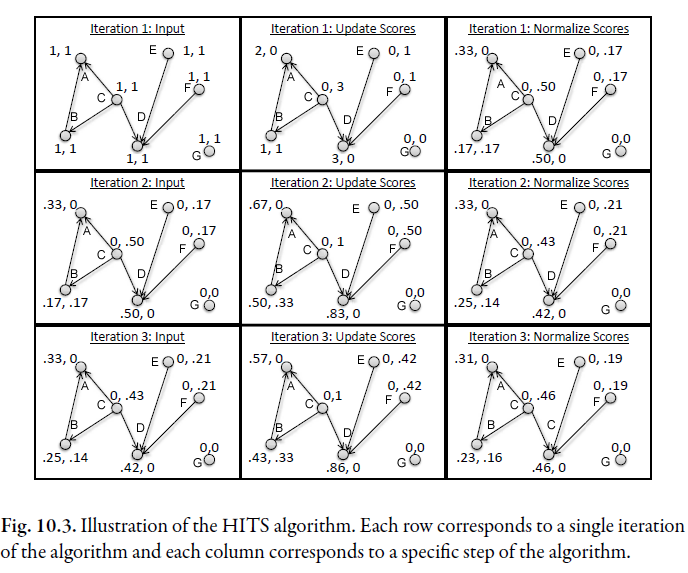
\includegraphics[scale=0.45]{images/fig-10-3.png}
\end{center}
\end{figure}

\subsection{Approach}
Vertices identification was added to the graph in order to better reference the nodes for further analysis. Graph $G$  on Figure \ref{fig:10.3} is composed of the following vertices: \{A, B, C, D, E, F, G\}.
\subsubsection{HITS}
To calculate 5 iterations of the HITS algorithm for the graph shown on Figure \ref{fig:10.3}, the \textit{Python} scripts \textit{hits.py} was developed (See Listing \ref{listing:hits}). The data structure to construct the graph is a dictionary, shown on lines 30 through 36. Each \textit{vertex} in the graph has another dictionary whose value contains the authority and hub score calculated during the iteration. The \textit{vertex} has an outbound connection to another on. A dictionary with the key value 'o' has an array containing all outbound \textit{vertices} connections. An additional dictionary, \textbf{node\_value} on line 37, has the authority and hub tuple initial iteration values. The remaining lines are the implementation of the algorithm provided in textbook \cite{CroftMetzlerStrohman}



\lstinputlisting[language=Python,
                 style=mybox, 
                 captionpos=t,
                 caption={Script Generate $n$ Number of HITS Iterations},
				 linerange={28-62},
				 firstnumber=28,                  
                 label=listing:hits,
                 ]
{../hits.py}

\subsubsection{PageRnk}
To calculate five iterations of the PageRank algorithm for the graph shown on Figure \ref{fig:10.3}, we developed the \textit{Python} scripts  \textit{pagerank.py}. It has a difference the data structure as the one implemented in \textbf{HITS}. Here the \textit{vertices} contain the values of the inward connection with them. Also, the dictionary contains a key \textit{size} indicating the number of outbound connections, and the key \textit{pr} indicating the calculated PR scored during the iteration. Additionally, the PR score at the beginning of the iteration is captured in the dictionary \textbf{pr} on line 45.
\lstinputlisting[language=Python,
                 style=mybox, 
                 captionpos=t,
                 caption={Script Generate $n$ Number of PageRank Iterations},
				 linerange={20-58},
				 firstnumber=20,                  
                 label=listing:pagerank,
                 ]
{../pagerank.py}

\newpage
\section{Solution}
Looking at Figure \ref{fig:hits-pagerank}, we can find some similarities and difference between \textbf{HITS} and \textbf{PageRank} algorithm results. In the HITS algorithm at the fifth iteration, \textit{vertex} \textbf{D} shows the highest authority score, similarly the same \textit{vertex} has the highest PR rank scored through the same number of iterations. The same was noticed for \textit{vertex} B, which has the second highest authority rank scored on the \textbf{HITS} algorithm. It also has the second high PR score in the \textbf{PageRank} algorithm. \\

\textbf{PageRank} seemed to converged at the third iteration while \textbf{HITS} appeared to converged at the fifth iteration.\\

\textbf{HITS} providesa more descriptive information about why a particular node is important. It tells  whether a node is providing information as an authority, or whether it is a hub  pointing to the correct authority.\\

In \textbf{PageRank}, \textit{vertex} G has a very small PR score even-though G is not connected to any of the other nodes in the graph. This is due to the $\lambda$ factor or the damping factor which, in our case, was set to 0.15.  However, the same \textit{vertex} shows no scores, either as an authority or as a hub.
\begin{figure}[H]
\caption{Result After 5 Iterations for HITS and PageRank Algorithms}
\label{fig:hits-pagerank}
\centering
\begin{subfigure}{.5\textwidth}
  \centering
	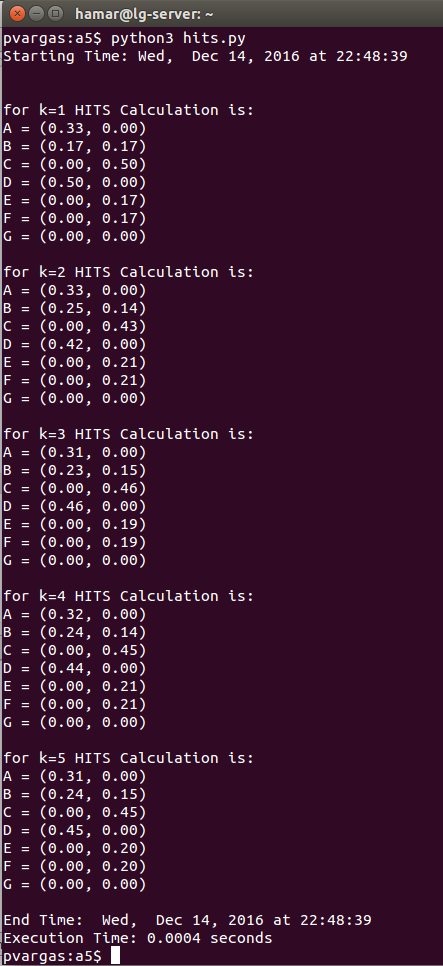
\includegraphics[scale=0.45]{images/hits.png}
  	\caption{HITS 5 Iteration Calculation Results}
	\label{fig:hits}  \label{fig:sub1}
\end{subfigure}%
\begin{subfigure}{.5\textwidth}
  \centering
  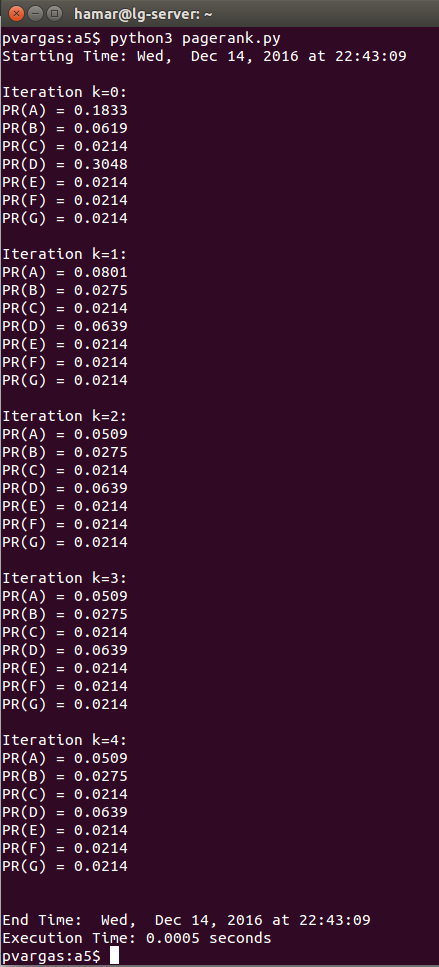
\includegraphics[scale=0.45]{images/pagerank.png}
  \caption{PageRank 5 Iteration Calculation Results}
  \label{fig:pagerank}
\end{subfigure}
\end{figure}

\end{homeworkProblem}

%----------------------------------------------------------------------------------------
%	Problem 2
%----------------------------------------------------------------------------------------
%\begin{homeworkProblem}[Exercise 10.6]% Custom section title
%\vspace*{10pt} % Question
%Find two examples of document filtering systems on the Web. How do they
%build a profile for your information need? Is the system static or adaptive?
%
%\end{homeworkProblem}
%
%----------------------------------------------------------------------------------------
%	Problem 3
%----------------------------------------------------------------------------------------
%\begin{homeworkProblem}[Exercise 10.9]% Custom section title
%\vspace*{10pt} % Question
%Both the clustering and nearest neighbor–based collaborative filtering algorithms
%described in this chapter make predictions based on user/user similarity.
%Formulate both algorithms in terms of item/item similarity. How can the distance
%between two items be measured?
%
%\end{homeworkProblem}
%----------------------------------------------------------------------------------------
%	Extra Credit SVM Light
%----------------------------------------------------------------------------------------
\begin{homeworkProblem}% Custom section title
\vspace*{10pt} % Question
Using \url{http://www.cs.cornell.edu/People/tj/svm_light/
} work through the ``Inductive SVM'' example, discuss in detail the steps and resulting output.\\
\vspace{5mm}\\
The ``Inductive SVM'' example from \cite{svm} used the Reuters-21578 collection. 1000 positive and 1000 negative examples were used for the machine-learning  training, in order to determine if a particular document in the collection should be classified as ``corporate acquisition''. A test file $<test.dat>$ representing 600 documents, it served as the input to evaluate the accuracy of the created model.\\

\subsection{Input File Format} \label{sec:file-format}
The training file has the form:
\begin{verbatim} 
<line> .=. <target> <feature>:<value> <feature>:<value> ... <feature>:<value> # <info>
<target> .=. +1 | -1 | 0 | <float> 
<feature> .=. <integer> | "qid"
<value> .=. <float>
<info> .=. <string> 
\end{verbatim}

Considering that the \textbf{positive} and \textbf{negative} examples are included in a single file, in order to distinguish if the training document is for a positive example, the value of \textbf{1} is placed at the beginning of the record. On the contrary, a \textbf{-1} value indicates the training record is related to a negative example.\\

In order to create our prediction model, the following instruction should be placed in the command-line:
\begin{center}
\textbf{svm\_learn example1/train.dat example1/model}
\end{center}

\begin{figure}[H] \label{fig:svm-trn}
\begin{center}
\caption{Training Module}
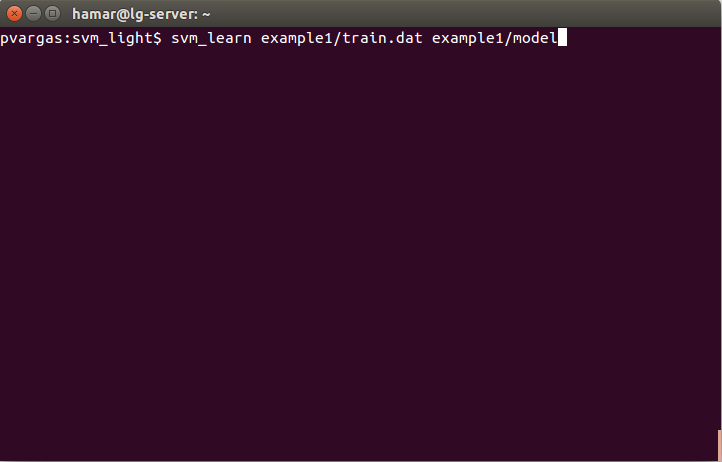
\includegraphics[scale=0.45]{images/svm-training.png}
\end{center}
\end{figure}

\newpage
\subsection{Resulting Output}
The accuracy of the report is shown on Figure \ref{fig:svm-trn-result}

\begin{figure}[H] 
\caption{Data Training Result}
\label{fig:svm-trn-result}
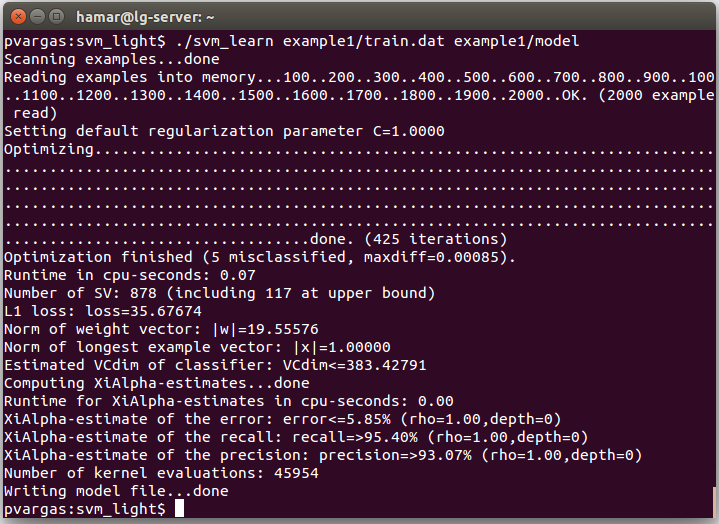
\includegraphics[scale=0.45]{images/svm-trn-result.png}
\end{figure}

\subsubsection{Number of SV}
Although the entire collection has \textbf{9,947} words, the number of features required to make the classification for any particular document in the collection as a ``corporate acquisition'' was calculated at:
$SV = \textbf{878}$. 
Therefore, the model only requires \textbf{878} features to obtain our classification.

\subsubsection{Loss Function}
Measurement of empirical error, define the error the classifier made on the training set. 

\subsubsection{Norm of Weight Vector}
According to \cite{CroftMetzlerStrohman},  
for all document pairs in the rank data, we would like the
score for the document with the higher relevance rating (or rank) to be greater
than the score for the document with the lower relevance rating. For our data $|x|= 19.55576$.

\subsubsection{VC Dimension Result}
The VC dimension or \textbf{Vapnik–Chervonenkis dimension} measures the number of points required to shatter  the classification model. For this example:
$VCdim <= \textbf{383.42791}$

\newpage
\subsubsection{Testing the Model}
Looking at Figure \ref{fig:svm-test-result}, we can see that 14 out of 600 documents were incorrectly predicting, bringing the accuracy of this model to \textbf{97.6\%} accuracy. This error falls into the predicted \textit{XiAlpha-estimate} error of less than 5.85\%.
\begin{figure}[H] 
\caption{Data Test Result}
\label{fig:svm-test-result}
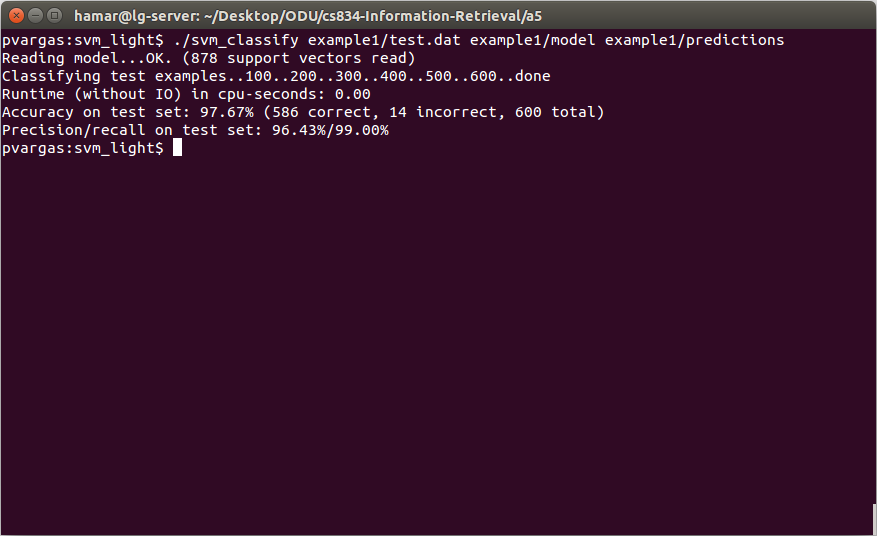
\includegraphics[scale=0.40]{images/example-result.png}
\end{figure}
\end{homeworkProblem}

%----------------------------------------------------------------------------------------
%	Extra Credit
%----------------------------------------------------------------------------------------
\newpage
\begin{homeworkProblem}% Custom section title
\vspace*{10pt} % Question
\begin{itemize}
\item create your own example modeled after the ``Inductive SVM'' example
\item pick a topic (e.g., ``Australia'') and provide 100 positive and 100 negative examples for training data:
	\begin{enumerate}[a. ]
		\item using the Reuters-21578 collection (linked from the SVMlight page)
		\item or, create your own collection with crawled web pages 
	\end{enumerate}
\item pick 30 documents not in the training set for your test data
\item stem the words in the collection, using TFIDF as the features (compute for the 230 documents)
\item train, classify, and discuss the results
\end{itemize}

\subsection{Approach}
\subsubsection{Topic Selection}
The collection selected for this exercise was \textbf{Reuters-21578}. This collection was accessed via the python library \textbf{nltk.corpus}. The topic chosen was ``\textbf{exports}.'' In order to obtain 100 positive examples for data training,  a \textit{Python} function was creating. The script \textit{svm-light.py} contains this function (\textit{find\_features}) which is shown on Figure \ref{listing:find-feature}.\\

\subsubsection{Selecting Positive Example Documents}
The first line for all the documents in the corpus is the title, which  is representative its content. The function \textit{find\_features} takes for argument a string, which is the term scanned in the document title (line 140). In order to obtain a document with plenty features, a minimum length of 500 characters was required for the document size to be considered for selection. The number of documents in the corpus under this criteria came out to be \textbf{136}.\\

The function returns an array containing the index for all the documents in the corpus where the term appears. The content of those documents were visually inspected for validity, and the first 100 indexes were stored in a file: \textit{positive.dat}. Later on, this file was going to be used as a input for the 100 positive training data examples. 

\lstinputlisting[language=Python,
                 style=mybox, 
                 captionpos=t,
                 caption={Scan for Feature in Document Title},
				 linerange={132-151},
				 firstnumber=132,                  
                 label=listing:find-feature,
                 ]
{../svm-light.py}
%
\vspace{10mm}
\subsubsection{Selecting Negative Example Documents}
A similar approach was used to obtain the negative training examples. The term ``\textbf{bank}'' was entered as the feature into the function \textit{find\_features}. The result was an array of 229 document indexes. The first 100 documents were viewed for content accuracy. In this case, it was ensured the content was not related to the term \textbf{export}. The document indexes were saved into the file: \textit{negative.dat}.

\subsubsection{Selecting Testing Documents}
Considering that only 100 indexes from 136 available were taken to be trained as positive examples, and the next 15 indexes were selected to serve as input for the testing data.  The same was done to find negative documents for the testing stage. In total, 30 documents were used for testing: 15 positive and 15 negative. The indexes for those documents were saved under the files: \textit{positive-test.dat}  and \textit{negative-test.dat} respectively.

\subsubsection{Building Word Index}
The online resource on \cite{svm-example} was very useful to stem the words in the collection. The PorterStemmer function from the \textbf{nltk} library facilitated the stemming action. The function \textit{create\_vocabulary} completed the stemming task. The function shown on Listing \ref{listing:stemming} reads all the documents in the corpus, then it tokenized each of the document and it placed the stemmed word into a set object(lines 305-306). Considering that the set does not have duplicate elements, the resulting set becomes the vocabulary. Its content was written to the file: \textit{words}.

\lstinputlisting[language=Python,
                 style=mybox, 
                 captionpos=t,
                 caption={Stemming Words in the Collection},
				 linerange={301-310},
				 firstnumber=301,                  
                 label=listing:stemming,
                 ]
{../svm-light.py}

\subsubsection{Creating Training Feature Records}
\textbf{$SVM^{light}$} requires the training input file in a specific format, as it is shown in section \ref{sec:file-format}. The resource cited on \cite{svm-example} contained a function that calculates \textbf{TFIDF} which is the value for the features in our training document. This function named \textit{tf\_idf} was incorporated into the script \textit{svm-light.py}, and it takes a string as a parameter, which in our case, it is the entire document. This function generates a \textbf{TfidVectorizer} object available in the  \textbf{sklearn.feature\_extraction} library. \\

The function \textit{tf\_idf} calls the function \textit{feature\_values} prior to passing the calculated vector. This last function takes all elements in the vector and converts them into a set of tuples ($w, v$), where $w$ is the tokenized word, and $v$ is its calculated \textbf{TFIDF} value.\\

Finally, the function \textit{write\_train\_data}, shown on Listing \ref{listing:training-data}, for each index marked as positive or negative in the  training files, \textit{positive.dat} and \textit{negative.dat} respectively, is opened and passed as an argument to the \textit{tf\_idf} (line 113). The returned tuples ($w, v$) are placed into a dictionary (lines 119-120), where the word $w$ is converted to the index in the vocabulary.\\

Since \textbf{$SVM^{light}$} requires the features to be placed in ascending order, the dictionary is sorted by key value prior to writing the features into \textit{train.dat}, which it is the file that it will be used for training data.

\lstinputlisting[language=Python,
                 style=mybox, 
                 captionpos=t,
                 caption={Creating Training Data},
				 linerange={102-129},
				 firstnumber=102,                  
                 label=listing:training-data,
                 ]
{../svm-light.py}

\subsection{Solution}
\subsubsection{Training $SMV^{light}$}\label{sec:prediction}
To create our model, we typed the command \textbf{svm\_learn train.dat model}, as it is shown on Figure \ref{fig:get-model}. The file \textit{train.dat} is the training data, and \textit{model} is the file that resulted from the machine learning. The estimated error is within \textbf{3\%}, therefore we are expected to have an accuracy greater or equal to \textbf{97\%}.
\begin{figure}[H] 
\caption{Data Training Result}
\label{fig:get-model}
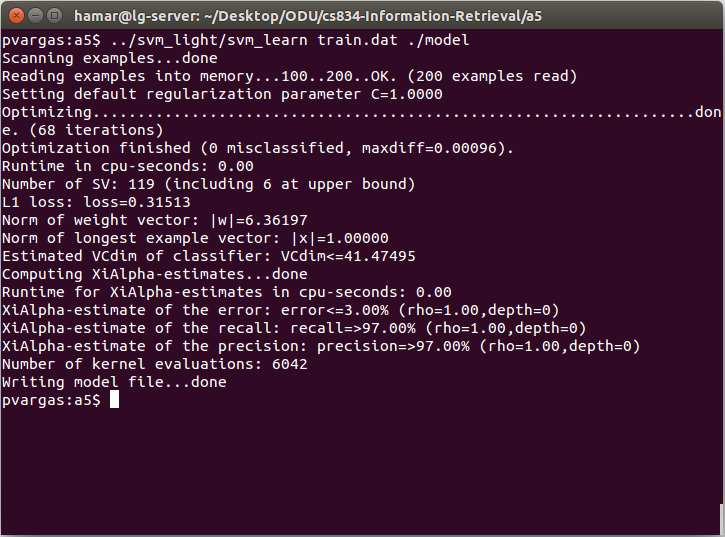
\includegraphics[scale=0.45]{images/smv-model.png}
\end{figure}

\subsubsection{Testing the Model}
To run the test, we typed the command \textbf{svm\_classify test.dat predictions}, as shown on Figure \ref{fig:test-result}. The file \textit{test.dat} contained the test data, and \textit{predictions} is the file that resulted after running the classification application. The accuracy of our test came out to be   \textbf{100\%}, which  agrees with the prediction on section \ref{sec:prediction}, which predicted that the results should be greater than or equal to \textbf{97\%}.

\begin{figure}[H] 
\caption{Testing Results}
\label{fig:test-result}
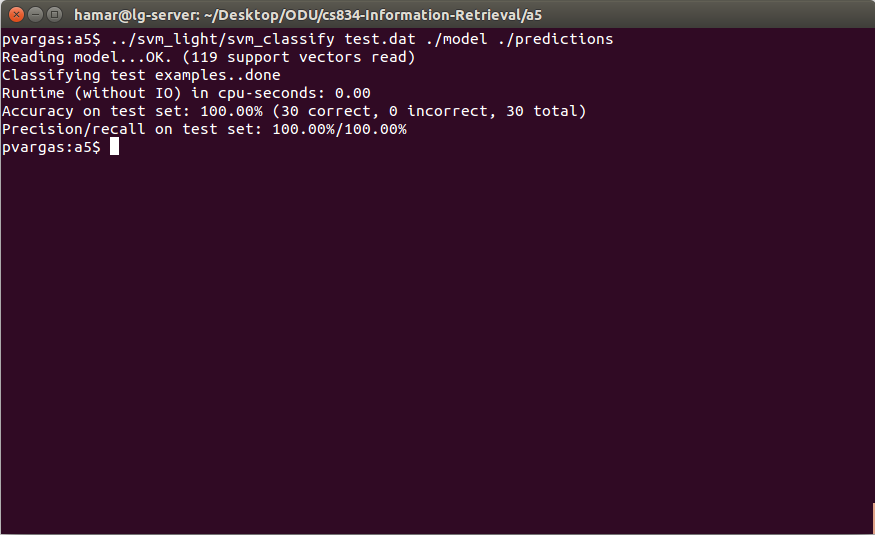
\includegraphics[scale=0.45]{images/test-result.png}
\end{figure}
\end{homeworkProblem}
%----------------------------------------------------------------------------------------
%	Bibliography
%----------------------------------------------------------------------------------------
\newpage
\bibliography{bibliography}
\bibliographystyle{siam}
%\begin{thebibliography}{9}
%\bibitem{Lutz} 
%Lutz, Mark (2013). List and Dictionaries. \textit{Learning Python} (5th ed.). (pp. %262-263). Sebastopol, CA: O'Reilly Media.
%
%\bibitem{ci}
%Segarn, Toby. Programming Collective Intelligence. \textit{Building Smart Web 2.0 Application}. (pp 29-53). Sebastopol, CA: O'Reilly Media.

%\bibitem{sitemaps}
%Sitemaps Schema. (n.d.) Retrieved September 21, 2016, from \url{http://www.sitemaps.org/schemas/sitemap/0.9}

%\end{thebibliography}
\end{document}